\chapter{Introducción específica} % Main chapter title

\label{Chapter2}

%----------------------------------------------------------------------------------------
%	SECTION 1
%----------------------------------------------------------------------------------------
Este capítulo trata sobre los recursos tecnológicos de terceros que fueron utilizados en la producción del trabajo.

% Descripción de las plataformas tecnológicas que sostienen al trabajo
\section{Tecnologías utilizadas}

% docker
Para crear una arquitectura de microservicios se utilizó Docker, que es un software que permite el uso y creación de contenedores de Linux.
Un contenedor es una unidad que empaqueta el código de un programa junto con sus dependencias para aislar su funcionamiento.
Para crear un contenedor, el motor de Docker se vale de el concepto de imagen.
Las imágenes son entidades aisladas que corren como contenedores durante el tiempo de ejecución sobre el motor de Docker.
Es la plantilla que crea un contenedor.
Los contenedores son entonces, unas abstracciones de la capa de aplicación de los sistemas Linux, como se puede visualizar en la figura \ref{fig:ch2WhatContainer}.
Varios contenedores pueden correr en el mismo ordenador como procesos aislados en el espacio de usuario sin generar ningún tipo de interferencias entre si.
La principal diferencia con las máquinas virtuales, es que estas son una abstracción del hardware del ordenador, transformando una única computadora en varios servidores.
Los contenedores en cambio, utilizan el kernel del sistema operativo del ordenador físico, no se abstrae un kernel, solo el espacio de aplicación o de usuario.

% docker files
Docker puede ser utilizado para construir imágenes definidas por el usuario.
Para lograrlo se usa un Dokerfile, que es un documento de texto que contiene todos los comandos que un usuario utilizaría para ensamblar una imagen.
El programador puede correr automáticamente una serie de comandos en sucesión al ejecutar un único comando sobre el Dockerfile.
Otra capacidad adicional es subir la imagen a un repositorio para ser descargado directamente sobre el entorno de producción.
De esta manera se facilita el despliegue de la aplicación, faltaría solamente, orquestar los contenedores para que trabajen en conjunto. 

% docker compose
La orquestación necesaria para la etapa de despliegue se logra utilizando Docker Compose.
Que según se indica en su documentación \citep{WEBSITE:WhatDockerCompose}, es una herramienta para definir y correr aplicaciones de Docker de múltiples contenedores.
Permite utilizar un archivo \emph{YAML} para configurar los servicios de la aplicación.
Con esta tecnología se puede crear y comenzar todos los servicios de la configuración utilizando un único comando y finalmente se logra tener orquestada la solución.

\begin{figure}[h]
	\centering
	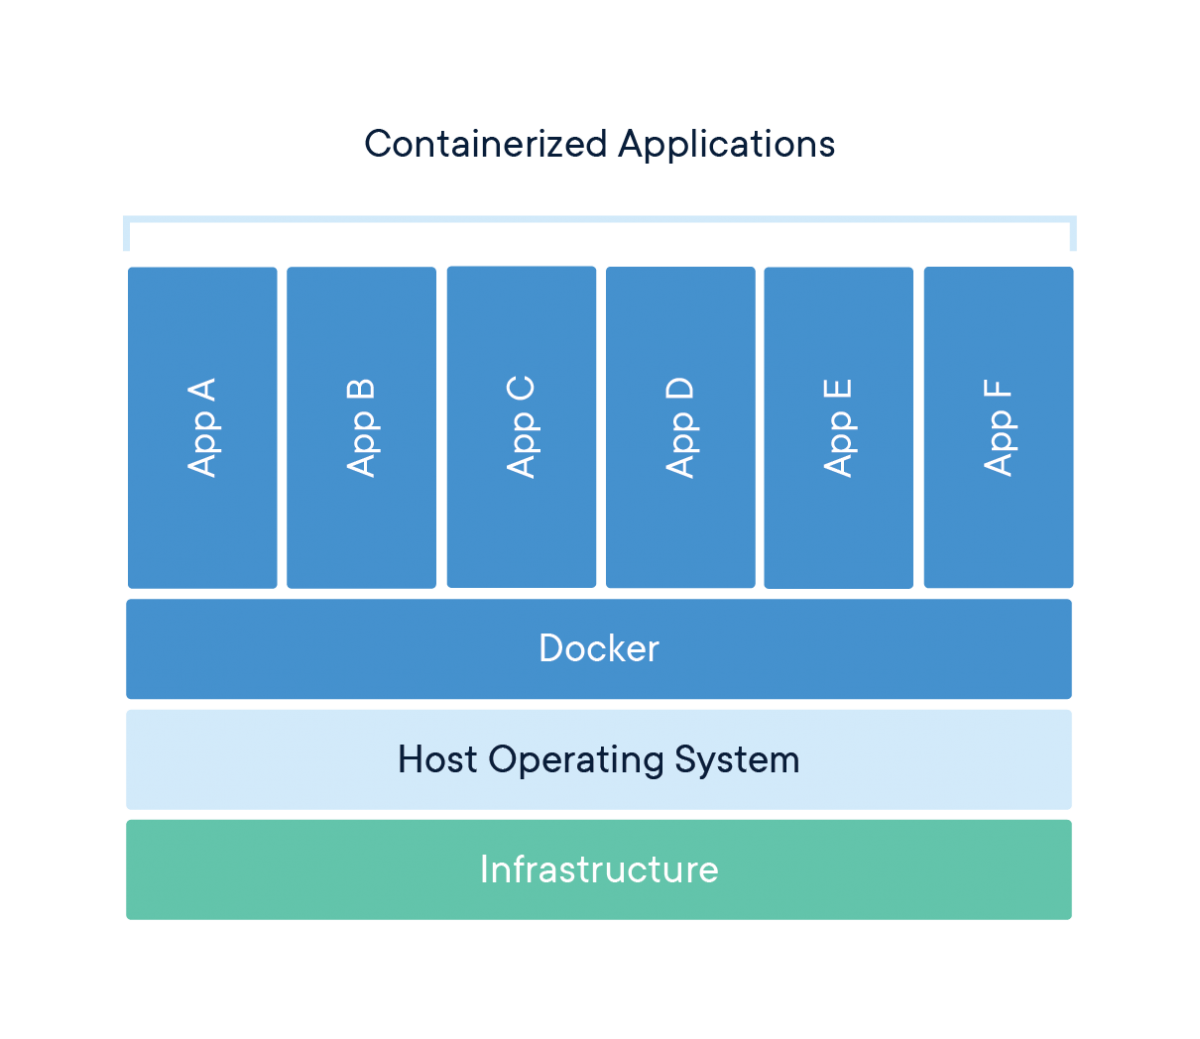
\includegraphics[width=\textwidth]{./Figures/ch2DockerContainer.png}
	\caption{Arquitectura de Docker. \citep{WEBSITE:WhatContainer}}
	\label{fig:ch2WhatContainer}
\end{figure}

% nodejs
El trabajo utiliza tecnologías web y la plataforma utilizada para implementarlas fue Nodejs, que es un servidor asincrónico y orientado a eventos que ejecuta JavaScript.
La orientación a eventos se consideró como una ventaja frente a las aplicaciones de concurrencia de múltiples hilos en el sistema operativo.
Principalmente porque no se utilizan candados y no existe la posibilidad de bloquear el servidor.
Una particularidad adicional es que fue diseñado para construir aplicaciones de red escalables y provee un gestor de paquetes muy fácil de utilizar.
Por estas razones y porque además fue una plataforma estudiada en la especialización, es que se la eligió para formar parte del trabajo.

% python
No todos los servicios del trabajo se realizaron con tecnologías relacionadas a JavaScript.
Particularmente se utilizaron una serie de bibliotecas y herramientas basadas en Python, que es un lenguaje de programación del tipo interpretado.
Este lenguaje posee una gran cantidad de recursos hechos por terceros y que se encuentran a disposición con licencias libres.
Si bien el lenguaje no fue visto con profundidad en la cursada, fue suficiente para entender su potencial.
Específicamente porque muchas de sus bibliotecas fueron útiles para desarrollar algunos servicios pequeños del trabajo.
Es una tecnología que resultó muy útil y fue utilizada para acelerar la creación de las partes más livianas del sistema. Partes que no justificaron el uso de una plataforma como Nodejs.

% mosquitto
Para implementar el protocolo MQTT se decidió utilizar paquetes y bibliotecas desarrolladas por terceros.
La primera herramienta fue Eclipse Mosquitto que es un broker del protocolo.
Es liviano, no demanda grandes recursos y puede ser ejecutado en ordenadores monoplaca.
Es flexible ya que permite ser configurado de distintas maneras según las necesidades de la aplicación.
Existen varios niveles de calidad de servicio para seleccionar y también se pueden agregar usuarios de manera opcional.
Los usuarios poseen distintos permisos para publicar y suscribirse a diferentes \emph{topics}.
También es posible utilizar una capa de seguridad en los mensajes que se basa en encriptación con llaves privadas y el uso de llaves públicas para realizar las lecturas.
Uno de los atractivos de la plataforma es la serie de programas utilitarios que incluye como recursos adicionales y que se integran en la terminal del sistema operativo.
Estas aplicaciones permiten realizar publicaciones y subscripciones para realizar pruebas y además se pueden crear contraseñas encriptadas para los usuarios.

% mongodb
Para persistir la información durante la ejecución del trabajo se utilizó MongoDB.
"MongoDB es una base de datos distribuida, basada en documentos y de uso general diseñada para desarrolladores de aplicaciones modernas y para la era de la nube". \citep{WEBSITE:MongoHome}
Se decidió utilizar esta tecnología para la capa de procesamiento debido a la afinidad que posee para realizar aplicaciones IoT.
Además es la base de datos documental más utilizada actualmente \citep{WEBSITE:DBRanking} y se evaluó como aspecto relevante, ganar experiencia con esta tecnología.

% redis
Los contenedores que forman la aplicación deben compartir una memoria volátil para que el trabajo pueda funcionar correctamente. Se eligió a Redis para que funcione como memoria compartida entre los componentes aislados del trabajo.
Redis es un almacén de estructuras de datos en memoria y puede ser usado como una base de datos, una \emph{caché} de memoria y un broker para crear un bus de eventos.
Esta tecnología permite hacer persistencia de datos pero solo en el esquema de clave-valor, permite también establecer tiempos de vida para los datos.
El tiempo de vida de los datos se utilizó en el trabajo para gestionar las sesiones de los usuarios, de tal manera que si una persona pasa demasiado tiempo sin interactuar con la aplicación deba volver a ingresar su usuario y contraseña para seguir utilizando el trabajo con normalidad.	
	
% Descripción de las dependencias del trabajo
\section{Bibliotecas y paquetes de terceros}

% Angular & Angular Material
Angular es un framework de diseño de aplicaciones para crear una SWA.
Se utiliza codificando en el lenguaje TypeScript que es un superset de JavaScript.
Está basado en el paradigma de componentes para generar aplicaciones escalables y poder reutilizar el código escrito en otros proyectos.
Pone a disposición una colección de bibliotecas para manejar formularios, comunicaciones cliente-servidor, \emph{routing}, entre otras.
Tiene entre sus facilidades ofrecidas, un cliente de terminal que acelera los tiempos de desarrollo.
Por todas estas ventajas, se decidió inclinarse por este framework.

Angular Material es una biblioteca de componentes de interfaz gráfica para Angular.
Está pensada para construir una experiencia consistente y funcional, adhiriendo con los principios de diseño más utilizados.
Estos principios se refieren a la portabilidad entre navegadores y la independencia de dispositivos.

% express & cors
Express es un framework para realizar servidores con Nodejs.
Está pensado para construir aplicaciones webs e interfaces de programación de aplicaciones (API).
Una API se encarga de definir las interacciones entre múltiples programas o puede intermediar entre componentes de hardware y software.
Express es la biblioteca más utilizada para trabajar con Nodejs. \citep{WEBSITE:Express}

% paho MQTT
Eclipse Paho es una biblioteca MQTT que está disponible para varios lenguajes.
En el trabajo realizado se utilizó para darle conectividad a los servicios programados en Python.
La biblioteca provee una clase cliente que habilita la comunicación con un broker MQTT, además provee funciones auxiliares que permiten codificar el código con mayor facilidad.

% mqttjs
MQTTjs es una biblioteca que provee de las herramientas para crear un cliente MQTT en Nodejs y en un navegador.
Se lo puede instalar de forma global en el sistema para hacer uso de las herramientas de terminal que ofrece.
Las herramientas permiten hacer pruebas de subscripción y publicación de mensajes.

% wsjs
ws es una biblioteca de Nodejs para realizar servidores con la capacidad de entablar una conexión WebSocket.
Es fácil de utilizar y es altamente configurable.
Se decidió usarla debido a que la documentación es completa y simple de entender.

% mongoose
Mongoose es una biblioteca de modelado de datos de objetos(ODM).
Se creó para trabajar con MongoDB y está disponible para la plataforma Nodejs.
El ODM gestiona las relaciones entre los datos, provee de una validación de esquema y se usa para traducir los objetos del programa en ejecución en una representación dentro de la base de datos.

% bcrypt jsonwebtoken
bcrypt es una biblioteca que contiene funciones para encriptar contraseñas.
La encriptación se basa en un esquema de \emph{hashing} e incorpora una \emph{salt} para proteger los datos de un ataque \emph{rainbow table}.
Para darle resistencia a los ataques de búsqueda por fuerza bruta, la biblioteca implementa una función adaptativa que por cada iteración se vuelve más lenta.
Esto hace que su resistencia sea fuerte aún cuando el ordenador que realiza el ataque sea potente.
Por estas razones se decidió usar este recurso en el trabajo para proteger las contraseñas de los usuarios.

% jsonwebtoken
jsonwebtoken es un paquete que permite crear un \emph{JavaScript Web Token (JWT)}.
JWT es un estandar que se utiliza para la fabricación de \emph{tokens} de acceso que permiten identificar una entidad y determinar cuales son sus privilegios en el sistema.
El token está formado por una cabecera, una carga útil y una firma.
La cabecera identifica el algoritmo de encriptación y el tipo de token.
La carga útil lleva consigo la información relevante para el funcionamiento.
Finalmente la firma cierra el token para certificar la llave privada del servidor.
Es relevante mencionar que la biblioteca está diseñada para funcionar con Nodejs

% chai & mocha
La biblioteca chai ofrece herramientas para hacer pruebas del software escrito.
Fue diseñada para Nodejs y puede ser integrada a cualquier framework de JavaScript.
En el trabajo fue combinado con Mocha, que es un framework de pruebas para Nodejs.
Las pruebas obtenidas al combinar estos dos recursos fueron fundamentales para detectar comportamientos no deseados.

% pyModbusTCP
Para que el código escrito en Python pueda utilizar el protocolo Modbus TCP se usó la biblioteca pyModbusTCP.
Este recurso permite crear un cliente para acceder a un servidor o bien crear una aplicación que se comporte como esclavo.

% oitc/modbus-server
oitc/modbus-server es un servidor Modbus TCP realizado en Python y disponible como imagen de Docker.
Está configurado para utilizar el puerto 5020 para evitar problemas de permisos con el sistema operativo. \citep{WEBSITE:dockerhubModbus}

% Descripción del sistema marca Honeywell que funciona en planta.
\section{Sistema propietario del cliente}

EBI es un sistema de automatización de edificios y gestión empresarial creado por la firma Honeywell.
Ofrece herramientas para dotar a las dependencias de las empresas de inteligencia para incrementar la comodidad, mejorar la seguridad y reducir los costos operativos.

La solución ofrece gestionar una red de edificios a través de una única interfaz gráfica. Pretende reducir los tiempos de respuesta frente a situaciones anormales y mejorar la seguridad.
Esta tecnología es compatible con dispositivos y software de terceros, con la idea de ofrecer escalabilidad.

Este software es un ecosistema de módulos que pueden ser adquirido a través de licencias para agregar las siguientes funcionalidades:

\begin{itemize}
	\item Gestión de consumo energético
	\item Seguridad de vida
	\item Control de acceso y intrusión
	\item Vídeo vigilancia
\end{itemize}

Las distintas licencias que ofrece Honeywell permiten que EBI utilice los protocolos BACNet, OPC, LonWorks y Modbus TCP.
Gador adquirió el producto con la licencia Modbus TCP para conectar sus PLCs de distintas marcas.
Como se puede observar en la figura \ref{fig:ch2EBI1}, se utiliza el software para visualizar los sensores de los distintos cuartos de producción y depósitos.
En la figura \ref{fig:ch2EBI2} se puede visualizar que EBI está a cargo del control ambiental de las plantas del cliente.
El sistema es el corazón de la gestión de edificios de la compañía.

\begin{figure}[h]
	\centering
	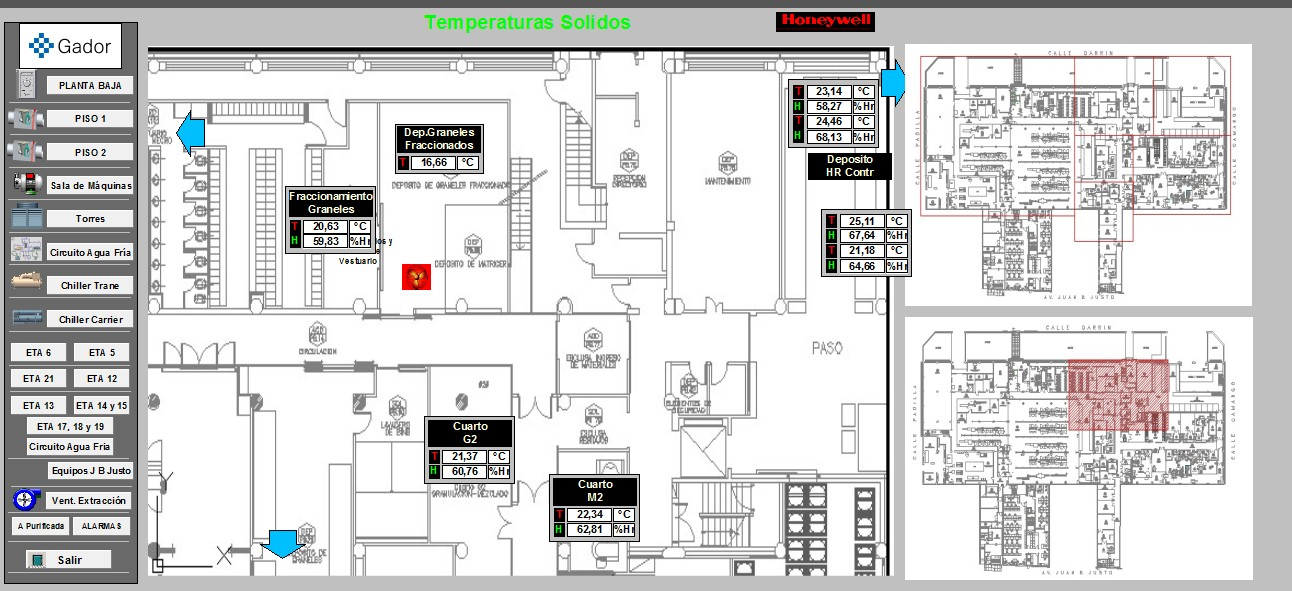
\includegraphics[width=\textwidth]{./Figures/ch2EBI1.jpg}
	\caption{Control de temperatura de sólidos.}
	\label{fig:ch2EBI1}
\end{figure}

\begin{figure}[h]
	\centering
	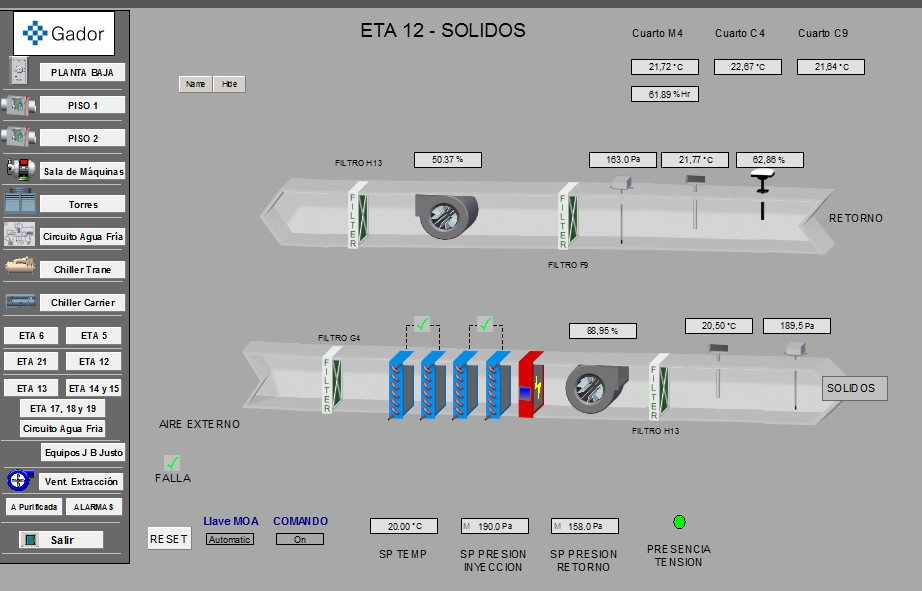
\includegraphics[width=\textwidth]{./Figures/ch2EBI2.jpg}
	\caption{Unidad de tratamiento de aire de sólidos.}
	\label{fig:ch2EBI2}
\end{figure}